\documentclass[11pt]{article}
\usepackage[margin=2cm,a4paper]{geometry}
\usepackage{graphicx}
\usepackage{amsmath}
\usepackage{amsfonts}
\usepackage{authblk}
\usepackage{float}
\usepackage{verbatim}

\usepackage[outdir=./img/]{epstopdf}
\usepackage{epsfig}
\usepackage{url}
%\usepackage[nomarkers,nolists,tablesfirst]{endfloat}

\usepackage{xr}
\externaldocument{supplement}
\usepackage{tikz}
\usetikzlibrary{fit,positioning}
\usetikzlibrary{arrows}

\setlength\parindent{0pt}

\begin{titlepage}
\title{\vspace{60mm} \bf
        Containerization of microbial protoeomics data processing pipelines
}  %Fix to center title vertically
\author{Timothy Bergström}
\maketitle
\thispagestyle{fancy}  %Page number for title (\maketitle clears foot and head, so it needs to be after it)
\vspace*{\fill}
\centering{tib@kth.se \\ KTH: Royal institute of technology}
\end{titlepage}


\begin{document}

\maketitle

{ {\bf Running Title -- } Parallelization and containerization of quantitative protoeomics data processing pipelines}

\begin{abstract}
The methods for processing shotgun proteomics data are not always straight forward to operate, and sometimes need manual intervention. This problem is exacerbate due to a preference toward UNIX among bioinformatician software developers, while instrument manufacturerers' with few exceptions operate under Windows. In practice, this means that many mass spectrometry labs use Windows computers just for making the format conversion. This also means that there will be software environment issues. Containerization enables installation of software into a virtual container environment, in a so-called container, as opposed to into a particular computer. The container can be distributed, while guaranteed to execute the exact same way regardless of operating system. In this paper we use \textit{Singularity} to contain a novel method developed in out lab, \textit{Quandenser} (QUANtification by Distillation for ENhanced Singals with Error Regulation), that increase the sensitivity of the LFQ analysis pipeline. This pipeline incorporates multiple processing steps, coded in separate executables. Among other tools, it contains Dinosaur, MaRaCluster, Crux, qvality and Triqler. To facilitate the installation of the method, all these components are placed in the Singularity container. To further facilitate the processing we used a workflow managing system, \textit{NextFlow}. We benchmark our method against established protein quantification method, \textit{MaxQuant} using \textit{Geyer}, \textit{Latosinska} and \textit{Bracht} data sets and find that our method has superior computational time. FIXME
In addition, it can be used in High Performance Computing clusters. Lastly, features for processing a novel scan method called \textit{BoxCar} has also been incorporated into our processing pipeline.

\end{abstract}

\section*{Introduction}
Mass spectrometry-based proteomics is currently seen as the most comprehensive technique to analyze protein content in biological samples. Modern MS generate vast amounts of data and the analysis of such data is generally considered as a bottleneck. This has its reasons. The methods for processing the data are complex and are not always straight forward to operate, and sometimes need manual intervention. As it is hard to recreate the exact software environment used during processing, many results produced with mass spectrometers cannot be accurately reproduced outside of the lab where it was initially generated.

The seemingly ever increasing performance of each generation of mass spectrometry equipment drives both sample sizes and the number of spectra per sample in a manner that the frequently single processor implemented approaches to data processing has a hard time to keep up.

There is also a mismatch between the bioinformaticians who often develop methods operating under Unix, and the fact that the instrument manufacturers' software with few exception operate under Windows. In practice this means that many mass spectrometry labs keep them selves with Windows computers, just for making format conversions between vendor specific raw file formats and non-proprietary file formats that can be read under windows.

The proteowizard community have created an windows executable that does such conversions. The system can be executed under the windows emulation program wine, however, the installation process is complicated and such installation are brittle and stop working over time.

New technology, so called containerization, provides means to install software, not into a particular computer, but into a virtual container environment, in a so-called container. The container can be distributed to several separate computers, yet is guaranteed to execute in the exact same way regardless of the operating system. There are several such containerization techniques available. The perhaps most popular one, docker, have a wide variety of available libraries of containers, and e.g. biocontainers \cite{FIXME}. However, docker containers, due to their nature, are executed with systems administrator privileges, and could be utilized for malicious purpose.  In this work we will focus on one named \textit{Singularity}, as it does not execute under root privileges and hence is the preferred solution of most computer cluster and High Performance Computing (HPC) clusters, particularly the ones in an academic environment.

Recently, the proteowizard community developed a docker-container for the wine implementation of msconvert (\url{https://hub.docker.com/r/chambm/pwiz-skyline-i-agree-to-the-vendor-licenses/}). This is tremendously helpful, as it enables linux developers to produce pipelines that can operate from beginning to end inside a Linux environment, or even an HPC environment.

We recently introduced a new method, {\em Quandenser} (QUANtification by Distillation for ENhanced Signals with Error Regulation), that increase the sensitivity of the LFQ analysis pipeline. Just as any proteomics data analysis method, the processing consist of multiple steps, coded in separate executables. Among other tools it contains Dinosaur\cite{teleman2016dinosaur} for feature finding, MaRaCluster\cite{the2016maracluster} for clustering, Crux\cite{mcilwain2014} for database searching, and qvality\cite{kall2008non} as well as Triqler\cite{the2018integrated} for error assessments. To facilitate the installation of the method we placed these components in a Singularity container.

To further facilitate the processing we used a workflow managing system, deals with how different pieces of dependent software can be consequently executed in a particular environment. Again, there are several workflow managers available, but the one used was \textit{NextFlow}\cite{di2017nextflow}.

Quandenser condenses the quantification data by applying unsupervised clustering on both MS1 and MS2 level and thereby paves the way for a quantification-first approach. The algorithm combines the unknowns from both levels into a condensed set of MS1 features and MS2 spectra that are likely to be interesting for further investigation. Specifically, Quandenser incorporates MBR for MS1 features to increase sensitivity and uses MS2 spectrum clustering to decrease the number of spectra to be searched. Importantly, it also provides {\em feature-feature match} error rates which can be used as input to Triqler to account for the errors as a result of the MBR step.

Here, we introduce \textit{Quandenser-pipeline}, a pipeline utilizing Nextflow as the workflow manager and all the software mentioned previously, packed into a Singularity container. The pipeline is able to be executed on HPC clusters which have Singularity installed and FIXME

\section*{Methods}

\subsection*{Data sets}
Three data sets consisting of RAW files were downloaded and tested on the pipeline, as well as compared with the performance of MaxQuant running the same data sets. The first data set was a subset of LFQ mass spectrometry data of patients before and after bariatric surgery (PRIDE id: PXD004242, 180 RAW files, total 97.5 Gb in size), which will be refered as the Geyer data set. The second data set was a study of Hepatitis C Virus-associated hepatic fibrosis (PRIDE id: PXD001474, 27 RAW files, total of 14.8 Gb) which will be refered as the Bracht data set and lastly, the third data set was from a study of bladder cancer using LFQ mass spectrometry data (PRIDE id: PXD002170, 8 RAW files, total 10.2 Gb in size) which will be refered as the Latosinska data set.

\subsection*{Processing data sets}
The pipeline and MaxQuant were processed on a computer running a Linux OS with an Intel i5-9600K (6 cores) @ 4.600GHz with 64 Gb of memory. MaxQuant version 1.6.3.3 and Quandenser-pipeline version 0.0821 was used to process the data sets. The fasta file used during processing the data was the reference proteome UP000005640 from Swissprot, accessed 2019-04-11. The setting "match-between-runs" in MaxQuant was enabled during processing. The pipeline was also tested on the HPC cluster Rackham at UPPMAX. The run time on the HPC cluster was adjusted by subtracting wait time between processes, due to the variation on SLURM waiting times during heavy load.

% BOSE
% Intel Core i7-4790k CPU @ 4.0 GHz with 32 Gb of memory.

\subsection*{User Interface}
To facilitate the operation of quandenser, we have provided quandenser with a user interface. The aim was to improve the usability of the workflow, to allow users to easily modify and run the pipeline to their choosing. Pyside2 was used to create the GUI, which is an GUI framework based by the Qt framework, with a LGPLv3 license \cite{pyside2}. To allow users to easily download and run the GUI from within the image, a shell script was created to minimize manual intervention and installation. The shell script installs Singularity, downloading the container from Singularity Hub and start the GUI embedded inside the image.

The new pipeline allows for an easy way of analyzing MS files with Quandenser, without requiring multiple dependencies and due to containerization of the software, it allows the pipeline to run on HPC clusters with Singularity as its only dependency. The pipeline also allows user to convert vendor files directly in the pipeline, minimizing the need to pre-convert the files before processing. The combination of faster processing time and being able to run on HPC clusters makes Quandenser-pipeline an excellent tool for analyzing label-free mass spectrometry data.

\section*{Results}

\subsection*{Parallelization}
In order to further reduce the running time, we investigated the possibilities to parallelize the processing within quandenser. Particularly we performed the following optimizations:
\begin{itemize}
  \item The conversion of each run from raw file-format into mzML-format is an embarrassingly parallelizable problem, in that each file can be processed in independent processes. We hence just enabled parallel processing by implementing the conversion process as a nextflow node. The result is a significant boost of performance during conversion, and is especially effective on HPC clusters where all files can be simultaneously converted.
  \item The initial feature finding with Dinosaur\cite{teleman2016dinosaur} can be done independently for each file. Again we could parallelize the process by putting this into a separate Nextflow node.
  \item Quandenser uses a minimum spanning tree strategy \cite{rost2016tric} to align the retention times of the different mass spectrometry runs. This makes an internal dependency structure. Every node in the minimum spanning tree will have to be aligned together with its sub-nodes, so the alignment process is done from the leafs inwards to the trunk.  However, at every level of the tree each branch can be processed independently. We have hence enabled individual processes to handle the alignment of every sub tree.
\end{itemize}

\subsection*{Run time comparison}
To demonstrate the processing speed of Quandenser-pipeline, we processed a couple of large-scale data sets. We compared the processing time some different platform needed to complete the processing of the data sets.

\begin{figure}[H]
  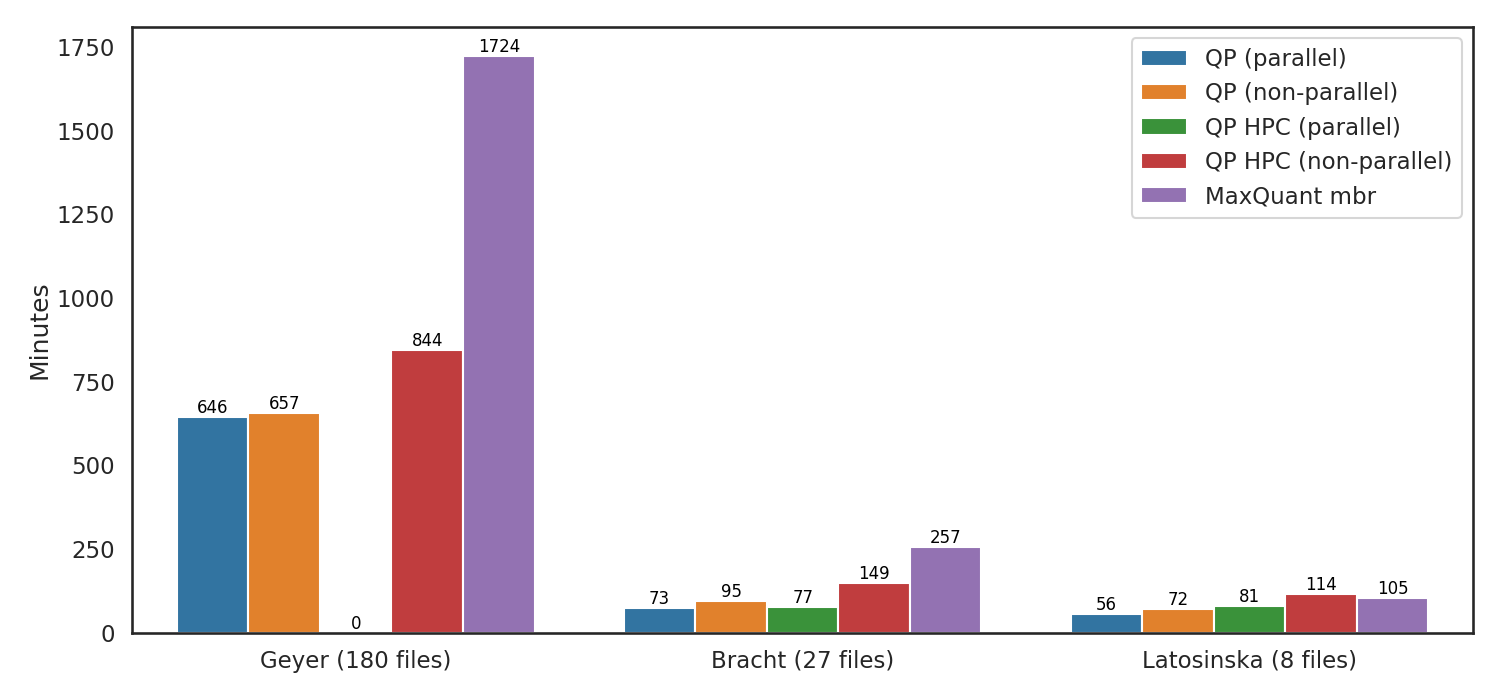
\includegraphics[width=\linewidth]{data/times.png}
  \caption{\textbf{Comparison of run time between the different quantification platforms reported in wall time.}}
  \label{fig:walltime}
\end{figure}

\begin{table}[!h]
  \begin{center}
  \caption{\textbf{Comparison of run time between the different quantification platforms reported in wall time.}}
  \label{table:walltime}
\begin{tabular}{lccc}
% This is from SHANNON, after the quandenser update
& Geyer & Bracht & Latosinska \\ \hline \hline
QP parallel (local) & 10h 46m & 1h 13m & 56m \\
QP non-parallel (local) & 10h 57m & 1h 35m & 1h 12m \\
QP parallel (HPC) & X & 1h 17m & 1h 21m \\  % Removed waiting time
QP non-parallel (HPC) & 14h 4m & 2h 29m & 1h 54m \\  % Removed waiting time
MaxQuant (local) & 28h 44m & 4h 17m & 1h 45m \\
\end{tabular}
\end{center}
\end{table}

\begin{table}[!h]
  \begin{center}
  \caption{\textbf{Comparison of run time between the different quantification platforms reported in cpu time in core hours}}
  \label{table:cputime}
\begin{tabular}{lccc}
% This is from SHANNON, after the quandenser update
% NOTE: Less core hours on local because each core is faster than in BOSE
& Weightloss & Bracht & Latosinska \\ \hline \hline
QP parallel (local) & 29.8 & 3.9 & 2.4 \\
QP non-parallel (local) & 16.9 & 3.0 & 1.8 \\
QP parallel (HPC) & X & 23.9 & 12.6 \\
QP non-parallel (HPC) & 210.9 & 29.0 & 18.2 \\
MaxQuant (local) & 103.7 & 15.5 & 6.2 \\
\end{tabular}
\end{center}
\end{table}

\section*{Discussion}
The performance of Quandenser-pipeline was significantly faster than MaxQuant on all data sets, FIXME\% faster for the FIXME data set.

A drawback with using parallel computation option of the pipeline is that the waiting time on the SLURM cluster for each process slows down the parallelization, meaning that a non-parallel run would be faster in some cases when the HPC cluster is under a heavy load.
On a local computer, the waiting time for each process is negligible, meaning a parallel processing would always be faster than non-parallel.

Another method of containerization is Podman, a daemonless container engine which solves some drawbacks with Singularity, one of which is that Singularity is read-only, while Podman containers can also write inside the container.

%Interesting discussion. Developer of Singularity chimes in on Podman Github
%https://github.com/containers/libpod/issues/3017

\bibliographystyle{plain}
\bibliography{pipeline}

\end{document}
